
% !TEX root = ../main.tex

% Local Variables:
% TeX-master: "../main"
% End:
% chktex-file 26

%%%%%%%%%%%%%%%%%%%%%%%%%%%%%%% Header %%%%%%%%%%%%%%%%%%%%%%%%%%%%%%%%%%%%%%%%%%%%
\begin{minipage}[l]{0.42\textwidth}
    
\includegraphics[width=1\textwidth]{img/logo-UNAMBA.png}
\end{minipage}
\hfill
\begin{minipage}[c]{0.5\textwidth}
    \begin{flushright}
	\large{\textbf{Unidad \#1}}\\
	\large{Lectures on Física III}\\
	\large{06 de octubre del 2025. Haquira, Apurimac}\\
        % \large{\textbf{Student:} Huallpa Aimituma Josué David}
    \end{flushright}
\end{minipage}
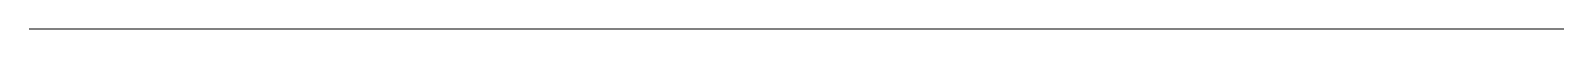
\begin{tikzpicture}
    \draw[gray,thick] (-5.5,0)--(14,0);
\end{tikzpicture}


 %%%%%%%%%%%%%%%%%%%%%%%% INICIO DEL CONTENIDO EN DOS COLUMNAS %%%%%%%%%%%%%%%%%%%%%
  
 \begin{multicols}{3}
    \begin{center}
         \LARGE{\textbf{Capítulo I: Electrostática}}\\	
         \vspace{1.2cm}
         % \Large {Lecturers Esteban Chalbaud \& Daniel Galviz} \\
         % \large{Teaching Assistant: Mauricio Gamonal \& Irvin Martínez}\\
         % \large{PhysicsLatam.com}\\
         % \vspace{1.2cm}
         \large{25 Septiembre 2025, 6:59 am (GMT-4)}\\
         % \vspace{1.2cm}
         \large{— Ficha de Trabajo —}
    \end{center}
    %%%%%%%%%%%%%%%%%%%%%%%%%%%%excercise%%%%%%%%%%%%%%%%%%%%%%%%%%%%%%%%%%%%%%%%
    \section{Capitulo noel}
Estructuralmente, Perl está basado en un estilo de bloques como los del C o AWK, y fue ampliamente adoptado por su destreza en el procesado de texto y no tener ninguna de las limitaciones de los otros lenguajes de script.La programación es el proceso de crear un conjunto de instrucciones (código) que una computadora puede ejecutar para realizar una tarea. Implica escribir, probar y mantener código en un lenguaje específico, como Python o JavaScript, para crear software y aplicaciones. La programación es fundamental para el desarrollo de la tecnología moderna, permitiendo la automatización de tareas y la creación de soluciones digitales
    
   


\end{multicols}
